\documentclass[a4paper,13pt]{scrartcl}
\usepackage[utf8]{inputenc}
\usepackage[french]{babel}
\usepackage{hyperref}
\hypersetup{unicode=true, pdftex, colorlinks=true, linkcolor=blue, citecolor=blue, filecolor=blue, urlcolor=blue, pdftitle=RIOT Cast the First Stone - French rules, pdfauthor=Ilario Gelmetti, pdfsubject=Riot Board Game}
\usepackage{graphicx}
\usepackage{tabularx}
\usepackage{geometry}

\geometry{
	top=1in,
	inner=1.4in,
	outer=1.4in,
	bottom=1in,
	headheight=2ex,
	headsep=2ex,
}
\setlength{\footskip}{30pt}



\renewcommand{\thesubsection}{\arabic{subsection}} % to remove the section numbers from subsections

\graphicspath{ {../img/} }

\title{RIOT - Jette la première pierre!}
\subtitle{Règles du jeu en francais}
\author{}
\date{}
\begin{document}

\maketitle

\url{https://noboardgames.com} 

%Para correcciones escribir a Ilario Gelmetti \texttt{ilario@eigenlab.org}

\section*{Contenu}
1 Plateau - 42 Cartes de Protestataires - 10 Cartes Opinion Publique - 2 Cartes de Mission pour les Nationalistes - 4 Cartons Récapitulatifs - 96 Jetons d'Unités

\section*{Le plateau}
Le Plateau représente en son centre le \textbf{Quartier Général de la Police (QG)}, pourvu d'un \textbf{Hôpital} ainsi que \textbf{6 Zones} délimitées par des bordures blanches. Chacune de ces Zones est divisée en: \textbf{Bâtiments} (produisant 1 ou 2 crédits), en \textbf{Rue} ainsi qu'en \textbf{deux Points d'Entrée} (le\textbf{ QG de la Police} et le \textbf{Point d'Entrée pour les Protestataires}).


\section*{Les équipes}
Dans RIOT vous avez le choix entre 4 différentes équipes: \textbf{La Police} et 3 différents types de \textbf{Protestataires}: les \textbf{Autonomes}, les \textbf{Anarchistes} et les \textbf{Nationalistes}.

\section*{Comment gagner}
Les conditions de victoire dépendent de votre choix d'équipe:
\begin{itemize}
\item La \textbf{Police} gagne quand la dernière carte «\textbf{Opinion Publique}» est retournée.
\item Les \textbf{Autonomes} et les \textbf{Anarchistes} gagnent quand ils arrivent à \textbf{7 Points de Zone}.
\item Les \textbf{Nationalistes} gagnent s'ils accomplissent la Mission Secrète qu'ils auront aléatoirement piochée au début de la partie.
\end{itemize}

\section*{Les cartes Opinion Publique (OP)}
Une Carte Opinion Publique est tirée à chaque fois que la \textbf{Police} est impliquée dans des \textbf{affrontements au corps à corps} avec un.e protestataire, peu importe l'issue du combat. A la fin du tour durant lequel a eu lieu l'affrontement, la carte est retournée et la police subit l'effet pénalisant qui y est inscrit. Par la même occasion elle se rapproche d'un pas vers la victoire (voir plus haut).

Une seule carte OP peut être révélée par tour  (ce qui signifie que dans une partie à 4 joueurs, un maximum de 4 cartes OP peuvent être révélées lors d'une manche complète) même si plus d'un affrontement valide a eu lieu. Toutefois, les différentes équipes protestataires peuvent s'affronter et se mettre sur la gueule sans pénalités (pour autant que la police ne soit pas impliquée).

\section*{Les Points de Zones}
Au début de leur tour, tant les \textbf{Autonomes} que les \textbf{Anarchistes} reçoivent un Point de Zone pour chaque \textbf{Zone} du plateau dont leurs unités occupent \textbf{tous les bâtiments}.

\section*{Les phases d'un tour}
\begin{enumerate}
\item Décompte des Points de Zone et des Crédits
\item Achat de cartes et recrutement d'unités
\item Déploiement d'unités
\item Déplacement des Unités et Usage des Cartes
\item Affrontements
\end{enumerate}

\subsection{Décompte des Points de Zone et des Crédits}
Au début de leur tour, tant les \textbf{Anarchistes} que les \textbf{Autonomes} vérifient s'ils/elles reçoivent des \textbf{Points de Zone}; Si tel est le cas, elles/ils mettent à jour le décompte sur leur \textbf{Carton Récapitulatif}. Les \textbf{Nationalistes} ne reçoivent pas de Points de Zone, mais reçoivent des Crédits pour les bâtiments qu'ils/elles occupent (voir plus bas).

Autonomes, Anarchistes et Nationalistes reçoivent des \textbf{Crédits} pour les bâtiment qu'elles/ils occupent; chaque bâtiment peut rapporter \textbf{1 ou 2 Crédits}, selon le chiffre indiqué sur le bâtiment même, indépendamment des Unités à l'intérieur.

Au début de son tour, la \textbf{Police} reçoit un Crédit pour chaque Unité ennemie restante (\textbf{Unités blessées} comprises) appartenant à l'équipe adverse qui en possède le moins.\\
Dans une partie à \textbf{3 joueurs/euses} la police reçoit aussi \textbf{+2 Crédits} à chaque tour.\\
Dans une partie à \textbf{4 joueurs/euses} la police reçoit aussi \textbf{+3 Crédits} à chaque tour.

\textbf{NB:} Vous ne pouvez pas collecter de Crédits entre deux tours, seulement après chaque manche complète.

\subsection{Acheter des cartes et recruter des unités}
Chaque Protestataire peut maintenant recruter des \textbf{Unités} et acheter des \textbf{Cartes} avec ses Crédits. La Police quant à elle ne peut que recruter des Unités.
Le coût de chaque Unité est indiqué sur les \textbf{Cartons Récapitulatifs}.
Le coût des \textbf{Cartes au sein d'un même tour} est progressif: la première Carte achetée coûte \textbf{1 Crédit}, la seconde \textbf{2 Crédits}, la troisième \textbf{3 Crédits}, etc.

\subsection{Déployer des unités}
Une fois qu'un.e joueur/euse a fini d'acheter des Cartes et de recruter des Unités, ces dernières doivent être déployées. Chaque joueur/euse place \textbf{ses nouvelles unités} sur les \textbf{Points d'Entrée} de son choix. La Police quant à elle doit toujours placer ses nouvelles unités dans son \textbf{Q.G.}

\subsection{Déplacer des unités et utiliser des cartes}
\subsubsection*{Déplacement}
Chaque Joueur/euse ne peut effectuer qu'\textbf{un déplacement à la fois}, de n'importe laquelle ou de toutes ses unités (sauf si elles profitent d'un bonus de mouvement), y compris les unités qui viennent juste d'être déployées et celles qui ont été blessées lors du dernier tour. Le premier mouvement d'une unité placée sur un point d'entrée (par exemple celles nouvellement recrutées ou blessées) s'effectue toujours vers la rue adjacente; une unité ne peut jamais s'arrêter sur un point d'entrée.
Les unités déjà présentes dans une rue peuvent se déplacer dans un bâtiment et donc par la même occasion l'occuper s'il était vide (ou l'attaquer s'il était déjà occupé par des unités d'une autre équipe). Pour ce faire la rue doit être vide de tout autre unité ennemie. Si ça n'est pas le cas, le/la joueur/euse ennemi.e peut choisir d'obstruer le mouvement, forçant le/la joueur/euse à abandonner le mouvement ou à démarrer un affrontement dans la rue. D'un autre côté, les unités peuvent se déplacer librement d'une rue à une autre ou d'un bâtiment à la rue adjacente, même si la rue de départ (ou la destination) est occupée par des unités ennemies. Les unités de la Police sont les seules à pouvoir entrer dans le QG de la police et à pouvoir le traverser (ce qui compte toutefois comme un déplacement).

\subsubsection*{Les cartes}
Les cartes peuvent être jouées à n'importe quel moment lors du tour d'un.e joueur/euse (avant, pendant et après la phase de mouvement) à l'exception des cartes Blitz (
\includegraphics[height=9pt]{blitz.png}) qui ne peuvent être jouées que lors d'affrontements dans lesquels le/la joueur/euse est impliqué.e.

\subsection{Affrontements}
Chaque unité peut attaquer n'importe quelle unité/ groupe d'unités situées à portée de ses possibles déplacements lors de ce tour.
Si une unité s'est déjà déplacée et n'est pas dans la même zone que sa cible, elle ne peut pas l'attaquer. Lors d'un affrontement, la force totale des unités concernées détermine le/la gagnant.e et le/la perdant.e; en cas d'égalité, rien ne se passe.
Chaque joueur/euse doit déclarer quelles unités prennent part à l'affrontement et qui en est la cible; le/la joueur/euse défenseur/euse doit utiliser toutes les forces présentes dans l'espace attaqué pour se défendre.
La police ne peut jamais déclencher une attaque lorsque ses unités sont inférieures aux unités protestataires dans l'affrontement.
Quand un.e joueur/euse défend un bâtiment, elle/il reçoit un bonus de +1 en force. Un groupe d'unités peut être attaqué un maximum de deux fois lors du tour d'un.e même joueur/euse.

Les affrontements sont divisés en deux phases: les attaques à distance et les attaques au corps à corps.

La phase d'attaque à distance peut commencer une fois que les unités participantes ont été déclarées: en commençant par la/le défenseur/euse, les deux joueurs/euses peuvent maintenant jouer leurs cartes Blitz (
\includegraphics[height=9pt]{blitz.png}) d'attaque à distance (voir attaque à distance); une fois que les effets des cartes ont été appliqués, l'attaquant.e peut choisir d'interrompre l'attaque ou de la poursuivre.
Si l'attaquant.e décide de poursuivre l'affrontement, on passe à la phase du corps à corps.
Lors de cette phase, les joueurs/euses peuvent utiliser tous les autres types de cartes Blitz; et l'affrontement est résolu en comptant la force totale des unités encore en place.
Le/la perdant.e retire toutes ses unités impliquées du plateau, tandis que le/la gagnant.e compte ses pertes et ses blessés/es (voir pertes et blessures).

\subsubsection*{Attaques à distance}
Lorsqu'un.e joueur/euse joue une carte Blitz d'attaque à distance lors d'un affrontement, il/elle décide immédiatement quelle unité ennemie cibler (à l'intérieur de ce groupe); cette unité reçoit immédiatement les dommages indiqués sur la carte; l'unité est alors retirée ou blessée, dans tous les cas elle ne pourra pas prendre partie aux phases suivantes de l'affrontement.

\textbf{NB 1:} Toutes les unités de police (mis à part l'unité de base) résistent au premier dommage d'une attaque à distance grâce à son bouclier (
\includegraphics[height=9pt]{shield.png}).
Cela veut dire qu'une carte d'attaque à distance +1 est inutile, tandis qu'une carte d'attaque à distance +2 ou deux cartes combinées d'attaques à distance +1 causeront 1 dommage.

\textbf{NB 2:} Si un affrontement auquel la police participe est résolu lors de cette phase (avec match nul ou avec des unités policières dans la minorité) il n'y a pas d'effets sur l'opinion publique.


\subsubsection*{Pertes et blessures}
Les unités victorieuses impliquées dans un combat reçoivent des dommages équivalent à la force totale des unités ennemies impliquées. Les dommages sont distribués en commençant par les unités avec le moins de force (en cas de force égale de celles qui ont un prix moindre). Une unité est blessée si les dommages qu'elle reçoit sont plus petits que sa force totale.
Les protestataires placent leurs unités blessées au point d'accès adjacent dans la zone où le clash a eu lieu; ils/elles reviennent dans la rue au tour du/de la joueur/euse suivant.e. La police place ses unités blessées dans l’hôpital; elles se déplaceront dans le QG au début du prochain tour du/de la joueur/euse et nécessitent donc deux déplacements pour retourner dans la rue.

\subsubsection*{Attaquer et défendre un bâtiment}
Comme mentionné plus haut, un bâtiment confère un bonus de +1 en force au/à la défenseur/euse.
Un.e assaillant.e ne peut pas utiliser de cartes Blitz d'attaque à distance contre des unités occupant un bâtiment, mais les defenseur/euses le peuvent.
Si l'assaillant.e remporte l'affrontement:toutes ses unités survivantes (y compris les blessées) entrent immédiatement dans le bâtiment.
Si le/la défenseur/euse remporte l'affrontement: toutes ses unités survivantes (y compris les blessées) restent à l'intérieur du bâtiment.

\section*{Premier tour de jeu}
En suivant un ordre aléatoire, chaque joueur protestataire pose une unité de base dans un bâtiment de son choix, jusqu'à ce que tout le monde ait deux bâtiments occupés dans deux zones différentes.

Jeu à deux joueurs/euses: Le/la joueur/euse protestataire place 4 unités dans 4 bâtiments dans 4 zones différentes.

Maintenant, la \textbf{Police} reçoit ses crédits et peut commencer son premier tour. A partir de maintenant la police pourra décider \textbf{à la fin de chaque manche} de l'ordre de jeu des joueurs/euses.

\section*{Unités spéciales}
\begin{minipage}[c]{0.2\textwidth}
\centering
\textbf{Mediactiviste}
\smallskip


\includegraphics[width=2cm]{special_units-mediaactivist.png}
\end{minipage}\hfill
\begin{minipage}[c]{0.75\textwidth}

\includegraphics[width=1cm]{po.png} Quand cette unité prend part à un combat il n'y a pas d'effet sur l'opinion publique.
\smallskip


\includegraphics[width=1cm]{card.png} Quand elle est éliminée en tant que défenseure, le joueur qui possède cette unité pioche immédiatement une carte.
\end{minipage}
\bigskip

\begin{minipage}[c]{0.2\textwidth}
	\centering
	\textbf{Black Bloc}
	\smallskip
	
	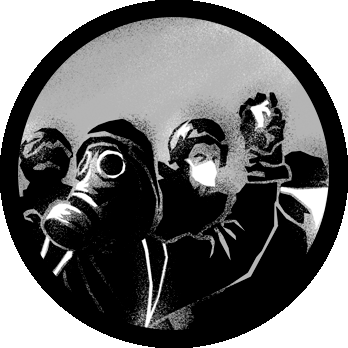
\includegraphics[width=2cm]{special_units-blackblock.png}
\end{minipage}\hfill
\begin{minipage}[c]{0.75\textwidth}
	
\includegraphics[width=1cm]{street.png} Quand cette unité combat dans la rue (ex.: pas en défendant ou en attaquant un bâtiment) sa force est de 3 (pour l'attaque et réception des dommages), dans tous les autres cas sa force est de 2.
\end{minipage}
\bigskip

\begin{minipage}[c]{0.2\textwidth}
	\centering
	\textbf{Paramilitaire}
	\smallskip
	
	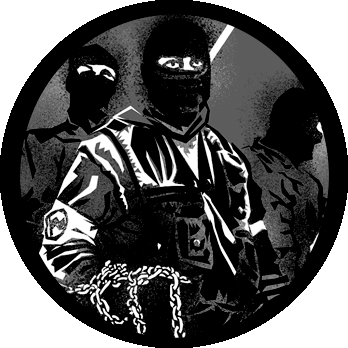
\includegraphics[width=2cm]{special_units-paramilitar.png}
\end{minipage}\hfill
\begin{minipage}[c]{0.75\textwidth}
	
\includegraphics[width=1cm]{direct_enter.png} Une fois recrutée, cette unité peut directement attaquer n'importe quel bâtiment occupé (si possible). Elle ne peut pas entrer dans un bâtiment vide, seulement en attaquer un occupé.
\end{minipage}
\bigskip

\begin{minipage}[c]{0.2\textwidth}
	\centering
	\textbf{Combi antiémeute}
	\smallskip
	
	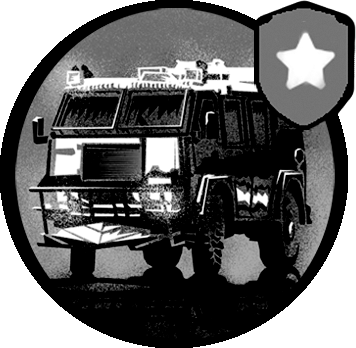
\includegraphics[width=2cm]{special_units-van.png}
\end{minipage}\hfill
\begin{minipage}[c]{0.75\textwidth}
	
\includegraphics[width=1cm]{movement.png} Cette unité peut effectuer deux déplacements à la place d'un seul, quand bien même elle serait à l'hôpital.
\end{minipage}
\bigskip

\begin{minipage}[c]{0.2\textwidth}
	\centering
	\textbf{R.A.I.D.}
	\smallskip
	
	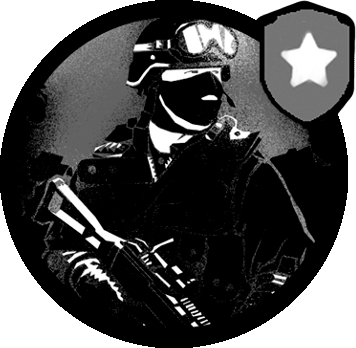
\includegraphics[width=2cm]{special_units-swat.png}
\end{minipage}\hfill
\begin{minipage}[c]{0.75\textwidth}
	
\includegraphics[width=1cm]{direct_enter.png} Une fois recrutées, cette unité peut directement attaquer n'importe quel bâtiment (si possible).
\end{minipage}

\end{document}
